% !TEX root = ../agglo_clust_review.tex

\renewcommand{\thesection}{A\arabic{section}}
\renewcommand{\thetable}{A\arabic{table}}
\renewcommand{\thefigure}{A\arabic{figure}}



\section{Appendix}

% Our code is available anonymously here: \url{https://anonymous.4open.science/r/GASP-4EDF}.

\subsection{Implementation and complexity of \algname{}} \label{sec:detailed_impl}



\paragraph*{Update rules} During the agglomerative process, the interaction between adjacent clusters has to be properly updated and recomputed, as shown in Algorithm \ref{main_alg}.  
An efficient way of implementing these updates can be achieved by representing the agglomeration as a sequence of \emph{edge contractions} in the graph. Given a graph $\mathcal{G}(V,E,\cost)$ and a clustering $\Pi$, we define the associated \emph{contracted graph} $\tilde{\mathcal{G}}_\Pi(\tilde{V}, \tilde{E}, \tilde{\cost})$, such that there exists exactly one representative node $|\tilde{V} \cap S| = 1$ for every cluster $S \in \Pi$ . Edges in $\tilde{E}$ represent adjacency-relationships between clusters 
and the signed edge weights $\tilde{\cost}_e$ are given by inter-cluster interactions $\tilde{\cost}(e_{uv})=\interact_{S_u \cup S_v}$, where $S_u$ denotes the clustering including node $u$. 
For the linkage criteria tested in this article, when two clusters $S_u$ and $S_v$ are merged, the interactions between the new cluster $S_u \cup S_v$ and each of its neighbors depend only on the previous interactions involving $S_u$ and $S_v$. Thus, we can recompute these interactions by using an \emph{update rule} $f$ that does not involve any loop over the edges of the original graph $\mathcal{G}$:
\begin{align}
  \interact(S_u \cup S_v  \cup S_t) =& f\Big[ \interact(S_u  \cup  S_t), \interact(S_v  \cup  S_t) \Big] \\
  =& f(\tilde{\cost}(e_{ut}), \tilde{\cost}(e_{vt})) 
\end{align}
In Fig. \ref{fig:edge_contraction_and_contr_graph} we show an example of edge contraction and in Table \ref{tab:linkage_criteria_explicit} we list the update rules associated to the linkage criteria we introduced in Table \ref{tab:linkage-criteria}.

\afterpage{ %
  \begin{algorithm*}[p]
    \caption{Implementation of \algname{} - Phase 1}
  \hspace*{\algorithmicindent} \textbf{Input:} $\mathcal{G}(V,E,w^+,w^-)$ with $N$ nodes and $M$ edges; boolean \texttt{{\color{blue}addCannotLinkConstraints}} \\
  \hspace*{\algorithmicindent} \textbf{Output:} Final clustering \\
    \hspace*{\algorithmicindent} 
    \begin{algorithmic}[1]
        \State $\tilde{\mathcal{G}}(\tilde{V},\tilde{E}) \gets \mathcal{G}(V,E,w^+,w^-)$  \Comment{Init. contracted graph}
        \State \texttt{UF} $\gets$ initUnionFind($V$) \Comment{Init. data structure representing clustering}
          \State PQ.push$(|w_e|, e) \quad \forall e \in E $  \Comment{Init. priority queue in desc. order of $|w_e|=|w_e^+ - w_e^-|$, $\mathcal{O}(|E|)$}
          \State \texttt{canBeMerged}$[e] \gets$ \texttt{True} $\,\,\, \forall e\in E$ \Comment{Init. cannot-link constraints}
      \State
        \While{PQ is \textbf{not} empty}
          \State $\tilde{w}, e_{uv} \gets $ PQ.popHighest() \Comment{$\mathcal{O}(\log |E|)$}
          \State \textbf{assert} \texttt{UF}.find($u$) $\neq$ \texttt{UF}.find($v$) \Comment{Edges in PQ always link nodes in different clusters}
          \If{({\color{green}\textbf{$\tilde{w} > 0$}}) \textbf{and} \texttt{canBeMerged}$[e_{uv}]$}
            \State PQ, \texttt{canBeMerged}, $\tilde{E}$ $\gets$ \textsc{UpdateNeighbors}($u,v$)
            \State $\tilde{V} \gets \tilde{V} \setminus \{ v\}$, $\quad \tilde{E} \gets \tilde{E} \setminus \{ e_{uv}\}$ \Comment{Update contracted graph}
            \State \texttt{UF}.merge($u,v$) \Comment{Merge clusters, $\mathcal{O}(\alpha(|E|))$}
          \ElsIf{({\color{red}\textbf{$\tilde{\cost} \leq 0$}}) \textbf{and} {\color{blue}\texttt{addCannotLinkConstraints}}}
            \State \texttt{canBeMerged}$[e_{uv}] \gets$ \texttt{False} \Comment{Constrain the two clusters}
          \EndIf
        \EndWhile
        \State
        \Return Final clustering given by union-find data structure  \texttt{UF}
    \end{algorithmic}
    \hspace*{1.5cm} 
      \begin{algorithmic}[1]
      \Function{UpdateNeighbors}{$u,v$}
        \State $\mathcal{N}_u = \{ t \in \tilde{V} | e_{ut}\in \tilde{E}  \}$
        \State $\mathcal{N}_v = \{ t \in \tilde{V} | e_{vt}\in \tilde{E}  \}$ 
        \For{$t \in \mathcal{N}_v$ } \Comment{Loop over neighbors in $\tilde{\mathcal{G}}$ of deleted node $v$}
          \State $\tilde{E} \gets \tilde{E} \setminus \{e_{vt}\}$
          \State $\tilde{w}_{vt} \gets$ PQ.delete($e_{vt}$) \Comment{Delete edge $e_{vt}$ from PQ and get the old edge weight, $\mathcal{O}(\log |E|)$}
          \State \texttt{canBeMerged}$[e_{ut}] \gets$ \texttt{canBeMerged}$[e_{ut}]$ \textbf{and} \texttt{canBeMerged}$[e_{vt}]$
          \If{$t \in \mathcal{N}_u$ }\Comment{Check if $t$ is a common neighbor of $u$ and $v$}
            \State $\tilde{w}_{ut} \gets$ PQ.delete($e_{ut}$)  \Comment{$\mathcal{O}(\log |E|)$}
            \State PQ.push($ |f(\tilde{w}_{ut}, \tilde{w}_{vt})|, e_{ut}$) \Comment{$\mathcal{O}(\log |E|)$  }
          \Else
            \State $\tilde{E} \gets \tilde{E} \cup \{e_{ut}\}$
            \State PQ.push($ |\tilde{w}_{vt}|, e_{ut}$) \Comment{$\mathcal{O}(\log |E|)$}
          \EndIf
        \EndFor
        \State
        \Return PQ, \texttt{canBeMerged}, $\tilde{E}$
      \EndFunction
    \end{algorithmic}
    \label{detailed_alg}
  \end{algorithm*}
  % \begin{figure*}[t]
  %         \centering
  %         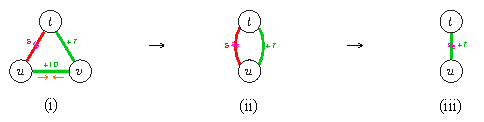
\includegraphics[width=0.7\textwidth]{./figs/proof_abs_max_example.pdf} % left bottom right top
  % \caption{\algname{} with \emph{AbsMax} linkage: Example representing the only case of edge contraction $e_{uv}$ that would introduce a positive attractive interaction between two constrained clusters. Note this can actually never happen with an \emph{AbsMax} linkage, because edge $e_{ut}$ has a lower absolute priority as compared to $e_{uv}$, so clusters $u$ and $t$ cannot have been constrained before $u$ and $v$ are merged. \TODO{Remove?}
  % }
  % \label{fig:abs_max_proof_example}  
  % \end{figure*}
  \begin{algorithm*}[p]
    \caption{Mutex Watershed Algorithm proposed by \cite{wolf2018mutex}}
  \hspace*{\algorithmicindent} \textbf{Input:} $\mathcal{G}(V,E,w^+,w^-)$ with $N$ nodes and $M$ edges \\
  \hspace*{\algorithmicindent} \textbf{Output:} Final clustering \\
    \hspace*{\algorithmicindent} 
    \begin{algorithmic}[1]
        \State \texttt{UF} $\gets$ initUnionFind($V$) 
        \For{$(u,v)=e\in E$ in descending order of $|w_e|=|w_e^+ - w_e^-|$}
          \If{\texttt{UF}.find($u$) $\neq$ \texttt{UF}.find($v$)} \Comment{Check if $u,v$ are already in the same cluster}
            \If{({\color{green}\textbf{$w_e > 0$}}) \textbf{and} \texttt{canBeMerged}($u,v$)}  \Comment{Check for cannot-link constraints}
              \State \texttt{UF}.merge($u,v$) and inherit constraints of parent clusters
            \ElsIf{({\color{red}\textbf{$w_e \leq 0$}})}
              \State Add cannot-link constraints between parent clusters of $u,v$
            \EndIf
          \EndIf
        \EndFor
        \State
        \Return Final clustering given by union-find data structure \texttt{UF}
    \end{algorithmic}
    \label{alg:mutex_watershed}
  \end{algorithm*}
  \clearpage
}


\paragraph{Implementation} Our implementation of \algname{} is based on an union-find data structure and a heap allowing deletion of its elements. 
In Phases 2 and 3, \algname{} is equivalent to a standard hierarchical agglomerative clustering algorithm with complexity $\mathcal{O}(N^2 \log N)$. In Algorithm \ref{detailed_alg}, we show our implementation of phase 1, involving cannot-link constraints.
In phase 1, the algorithm starts with each node assigned to its own cluster and sorts all edges $e\in E$ in a heap/priority queue (PQ) by their absolute weight $|\cost_e|=|w_e^+ - w_e^-|$ in descending order, so that the most attractive and the most repulsive interactions are processed first. It then iteratively pops one edge $e_{uv}$ from PQ and, depending on the priority $\tilde{\cost}_{uv}$, does the following: in case of attractive interaction $\tilde{\cost}_{uv}>0$, provided that $e_{uv}$ was not flagged as a cannot-link constraint, merge the connected clusters, perform an edge contraction of $e_{uv}$ in $\tilde{\mathcal{G}}_\Pi$ and update the priorities of new double edges as explained in Fig. \ref{fig:edge_contraction_and_contr_graph}. 
If, on the other hand, the interaction is repulsive ($\tilde{\cost}_{uv}\leq 0$) and the option \texttt{addCannotLinkContraints} of Alg. \ref{detailed_alg} is \texttt{True}, then the edge $e_{uv}$ is flagged as cannot-link constraint.


\begin{table}[t]
\centering
    \small
    % \vspace{-2em}
\begin{tabular}[t]{r | l }
            \toprule
            Linkage criteria & Update rule $f$ \\        
            \midrule
            Sum: & \thead[l]{$f(\tilde{\cost}_1,\tilde{\cost}_2) = \tilde{\cost}_1+\tilde{\cost}_2$} \\ 
            \makecell[r]{Absolute \\Maximum:} & \thead[l]{
            $
            f(\tilde{\cost}_1,\tilde{\cost}_2) = \begin{cases} 
            \tilde{\cost}_1 & \text{if}\,\, |\tilde{\cost}_1|>|\tilde{\cost}_2|\\
            \tilde{\cost}_2 & \text{otherwise}
             \end{cases} 
            $}
               \\ 
            \makecell[r]{Average:} & \thead[l]{$f(\tilde{\cost}_1,\tilde{\cost}_2) = \mathrm{weightAvg}\{ \tilde{\cost}_1, \tilde{\cost}_2 \} $}                 \\ 
            Single: & \thead[l]{$f(\tilde{\cost}_1,\tilde{\cost}_2) = \max \{ \tilde{\cost}_1, \tilde{\cost}_2 \}  $} \\
            Complete:& \thead[l]{$f(\tilde{\cost}_1,\tilde{\cost}_2) = \min \{ \tilde{\cost}_1, \tilde{\cost}_2 \}  $} 
        \end{tabular}\vspace{1em}
        \caption{The table lists the update rules $f(\tilde{\cost}_1, \tilde{\cost}_2)$ associated to the linkage criteria of Table \ref{tab:linkage-criteria} and that are used to efficiently update the interactions between clusters.}
\label{tab:linkage_criteria_explicit}  
\end{table}
\begin{figure}[t]
        \centering
        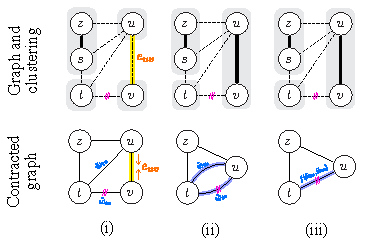
\includegraphics[width=0.48\textwidth]{./figs/edge_contraction.pdf} % left bottom right top
    \centering
    \caption{Example of edge contraction. First row: original graph $\mathcal{G}$; clustering $\Pi$ (gray shaded areas) with dashed edges on cut; cannot-link constraints (violet bars). Second row: contracted graph $\tilde{\mathcal{G}}_\Pi$. In step ii), edge $e_{uv}$ is contracted and node $v$ deleted from $\tilde{\mathcal{G}}_\Pi$. In step iii), double edges $e_{tu}$ and $e_{tv}$ resulting from the edge contraction are replaced by a single edge with updated interaction.}\label{fig:edge_contraction_and_contr_graph}  
\end{figure}



\paragraph*{Complexity} 
In the main loop of Phase 1, the algorithm iterates over all edges, but the only iterations presenting a complexity different from $\mathcal{O}(1)$ are the ones involving a merge of two clusters, which are at most $N-1$. By using a union-find data structure (with path compression and union by rank) the time complexity of \texttt{merge}$(u, v)$ and \texttt{find}($u$) operations is $\mathcal{O}(\alpha(N))$, where $\alpha$ is the slowly growing inverse Ackerman function. The algorithm then iterates over the neighbors of the merged cluster (at most $N$) and updates/deletes values in the priority queue ($\mathcal{O}(\log |E|)$). 
Therefore, 
similarly to a heap-based implementation of hierarchical agglomerative clustering, our implementation of \algname{} - Phase 1 has a complexity of $\mathcal{O}(N^2 \log N)$. In the worst case, when the graph is dense and $|E|=N^2$, the algorithm requires $\mathcal{O}(N^2)$ memory. Nevertheless, in our practical applications the graph is much sparser, so $\mathcal{O}(|E|)=\mathcal{O}(N)$. 
With a single-linkage, corresponding to the choice of the \emph{Maximum} update rule in our framework, the algorithm can be implemented by using the more efficient Kruskal's Minimum Spanning Tree algorithm with complexity $\mathcal{O}(N \log N)$, but only when cannotLinkConstraints are not used. 
Moreover, \algname{} with \emph{Absolute Maximum} linkage can be implemented more efficiently (see next section). %\TODO{Empirical complexity plot?}

\begin{figure}
% \vspace{-0.3cm}
\includegraphics[width=\linewidth]{figs/runtime-MWS.pdf}\\
% \vspace{-0.6cm}
\caption{Runtimes for different implementation of GASP with AbsMax linkage criterion. Runtimes are averaged over 5 runs.}
  \label{fig:runtimes_plot}
\end{figure}


\paragraph*{Efficiency of different GASP implementations with AbsMax linkage criteria} 
In Fig.~\ref{fig:runtimes_plot}, we compare the runtimes of three implementations of the AbsMax criteria: the implementation from \cite{wolf2019mutex} for pixel graphs (\emph{Pixel-grid implementation}) and for general graphs (\emph{Efficient graph implementation}) as well as the HC implementation with AbsMax linkage (\emph{Naive graph implementation}). The specialized implementations can exploit the properties of the underlying graph and are faster. But our generalization does not carry a large computational penalty and only requires a few extra seconds for partitioning graphs of a million nodes. Note that we have always used the most efficient implementation for the results reported in the paper. We will clarify this fact.

\paragraph{Median linkage} We implemented median linkage in our library from the beginning but did not report on it in the main paper for two reasons: we consider the other criteria to span the range of interesting behavior well; and it performs no better than some of the other criteria (like average linkage) which are faster to evaluate.
% Table~\ref{table:median_scores} compares average and median linkage on two clustering problems: 
% in terms of scores, the advantage of one linkage over the other seems to be application dependent, but the median linkage has higher runtime.

\begin{figure}
\includegraphics[width=\linewidth]{figs/counterexample_cropped.png}\\
\caption{GASP agglomeration with the Abs Max criterion: contracted edges are marked green. The last contraction increases the MC objective from -1 to 0.}\label{counterexample}
\end{figure}


\subsection{GASP relation to the multicut objective} \label{sec:relation_to_multicut}
For some of the linkage criteria, e.g. sum and average, GASP can be understood as a local search to the objective of the multicut optimization problem \ref{eq:MC_objective}, see \cite{levinkov2017comparative}. But this does not hold in general: the Abs Max linkage for example does not always decrease the MC objective (see counter example in Fig.~\ref{counterexample}). 
Moreover, GASP cannot be seen as a k-approximation, because it is a polynomial algorithm and \cite{chawla2006hardness} has shown that approximating the multicut objective with any constant factor is in itself NP-hard. 


\subsection{Proofs of Propositions \ref{prop:absmax_mutex}, \ref{prop:weight_shift_invariant}, \ref{prop:ultraMetric1}, and \ref{prop:ultraMetric2}}
\label{sec:proposition_proofs}

\begin{lemma} \label{lemma:absMax_and_complete_not_positive}
If \algname{} Algorithm \ref{main_alg} with \textbf{Complete linkage criteria} enforces a constraint between two clusters in \emph{Phase 1}, then the interaction between the clusters will never become positive over the course of the following agglomeration steps.
\end{lemma}
\begin{proof}
Two clusters are constrained in \emph{Phase 1} only if their interaction is repulsive and, with complete linkage,  the signed interaction between two clusters can only decrease over the course of the agglomeration. Thus, if two clusters are constrained by the algorithm, their negative interaction cannot increase and become positive later on in the agglomeration process.
\end{proof}

\begin{lemma} \label{lemma:absMax_and_complete_not_positive}
If \algname{} Algorithm \ref{main_alg} with \textbf{AbsMax linkage criteria} enforces a constraint between two clusters in \emph{Phase 1}, then the interaction between the clusters will never become positive over the course of the following agglomeration steps.
\end{lemma}
\begin{proof}
During the agglomeration the interaction between two clusters can only increase in absolute value. Thus, the negative interaction $\interact{}(S_i \cup S_j)<0$ between two constrained clusters can possibly become positive over the course of next agglomeration steps only if there is at least another pair of clusters in the graph that has a positive interaction $\interact{}(S_l \cup S_t)>0$ higher in absolute value: $|\interact{}(S_l \cup S_t)| > |\interact{}(S_i \cup S_j)|$.
If such clusters $S_l, S_t$ with positive interaction exist, we note that they must also be constrained (in the opposite case, the algorithm would have already merged them before to constrain $S_i$ and $S_j$, because their priority is higher). In other words, a constrained negative interaction can become positive only if there is already another positive constrained interaction: but this can never be the case because initially all constrained interactions are negative.
\end{proof}

\begin{lemma} \label{lemma:absMax_and_complete_property}
In the \algname{} Algorithm \ref{main_alg} with AbsMax or Complete linkage criteria (see linkage definition in Table \ref{tab:linkage-criteria}), the same final clustering is returned whether or not cannot-link constraints are enforced.
\end{lemma}
\begin{proof}
In phase 1 of Algorithm \ref{detailed_alg}, two clusters are merged only if the condition at line 9 is satisfied (i.e. when an interaction is both positive and not constrained). From Lemma \ref{lemma:absMax_and_complete_not_positive} and Lemma \ref{lemma:absMax_and_complete_not_positive} follows that with Complete and AbsMax linkage an interaction can never be both positive and constrained at the same time, so we directly conclude that the constrained and unconstrained versions of the algorithm will perform precisely the same agglomeration steps in phase 1.
In phase 2 (after constraints have been removed) no clusters are merged because all interactions are already negative (whether they previously constrained or not). Thus, both constrained and unconstrained versions of \algname{} return the same clustering $\Pi^*$.
\end{proof}

% We now prove Proposition \ref{prop:absmax_mutex}:

\absmaxmutex*

% \begin{prop} \label{prop:equiv_MWS}
% The Mutex Watershed Algorithm \ref{alg:mutex_watershed} (MWS) with empirical \linebreak $\mathcal{O}(N \log N)$ complexity introduced by \cite{wolf2018mutex} returns the same final clustering given by the \algname{} Algorithm \ref{detailed_alg} with the use of cannot-link constraints and an Absolute Maximum update rule:
% \begin{equation}\label{eq:def_abs_max}
% f_{\mathrm{Abs.Max.}}(\tilde{\cost}_1,\tilde{\cost}_2) = \begin{cases} 
%             \tilde{\cost}_1 & \text{if}\,\, |\tilde{\cost}_1|>|\tilde{\cost}_2|\\
%             \tilde{\cost}_2 & \text{otherwise}
%              \end{cases} 
% \end{equation}
% \end{prop}

% \paragraph{Remark on graph notation in \cite{wolf2018mutex}} The definition of a graph proposed by \cite{wolf2018mutex} makes a distinction between a set of positive edges $E^+$, associated with a set $W^+$ of positive scalar attributes representing merge affinities, and a set of negative edges $E^-$, associated with a set $W^-$ of positive attributes representing split tendencies. On the other hand, in our definition $\mathcal{G}(V,E,w^+,w^-)$ each edge have both an attractive $w_e^+$ and a repulsive $w_e^-$ attribute, so we can make them equivalent by defining:
% \begin{align}
% E^+ =&\,\, \{ e \in E \,\,\text{s.t.} \,\,w_e = w_e^+ - w_e^- > 0\}, \\
% E^- =&\,\, \{ e \in E \,\,\text{s.t.}\,\, w_e = w_e^+ - w_e^- \leq 0\}, \\
% W^+ =&\,\, \{ |w_e| \,\,\text{s.t.}\,\, e \in E^+\},\\
%  W^- =&\,\, \{ |w_e| \,\,\text{s.t.}\,\, e \in E^-\}.
% \end{align}


\begin{proof}%[Proof of Proposition \ref{prop:absmax_mutex}]
From Lemma~\ref{lemma:absMax_and_complete_property} it directly follows that \algname{} with AbsMax linkage criterion returns the same final clustering whether or not cannot-link constraints are enforced. In the following, we prove that MWS (see pseudocode \ref{alg:mutex_watershed}) and the constrained AbsMax version of \algname{} also return the same clustering.
Both algorithms sort edges in descending order of the absolute interactions $|w_e|$ and then iterate over all of them. The only difference is that MWS, after merging two clusters, does not update the interactions between the new cluster and its neighbors. 
However, since with an Abs. Max. linkage the interaction between clusters is simply given by the edge with highest absolute weight $|w_e|$, the order by which edges are iterated over in \algname{} is never updated. Thus, both algorithms perform precisely the same steps and return the same clustering.
% Next, we prove that \algname{} with AbsMax linkage method returns the same final clustering whether or not cannot-link constraints are enforced. In the \algname{} Algorithm \ref{detailed_alg}, the interactions between clusters are updated only when two clusters are merged and the condition at line 9 is satisfied (an interaction is both positive and not constrained). 
% We also observe that, in the unconstrained version of \algname{}, the predicate \texttt{canBeMerged} at line 9 can never be false because cannot-link constraints are never introduced at line 14. \TODO{Rephrase}
% Let us now contradict the initial hypothesis and assume by absurd that the constrained version of \algname{} introduces a cannot-link constraints between two clusters sharing a positive interaction $\tilde{w}>0$ and outputs a different clustering as compared to the unconstrained version. 
% This can happen only in the situation shown in Fig. \ref{fig:abs_max_proof_example}, when two clusters $u$ and $v$ are merged together and share a common neighboring node $t$ having the following two properties: a) $u$ and $t$ are already constrained and share a repulsive interaction $w_{ut}\leq0$, b) $v$ and $t$ share an attractive interaction $w_{vt}>0$ that is higher in absolute value $|w_{vt}|>|w_{ut}|$. 
% Then, according to Eq. \ref{eq:def_abs_max}, \TODO{} the new merged cluster $uv$ and $t$ are constrained and share a positive interaction. 
% But this case can never happen, since if $|w_{vt}|>|w_{ut}|$ then clusters $v$ and $t$ are merged before clusters $u$ and $t$ are constrained.  
\end{proof}
% \begin{prop} \label{prop:abs_max_cannot_link_property}
% The \algname{} Algorithm \ref{detailed_alg} with the Absolute Maximum linkage defined in Eq. \ref{eq:def_abs_max} returns the same final clustering whether or not cannot-link constraints are enforced. 
% \end{prop}
% \begin{proof}
% \end{proof}

% \subsubsection{Weight-shift invariance of \algname{} algorithms}
\begin{figure}[t]
% \begin{subfigure}[t]{0.48\textwidth}
\centering
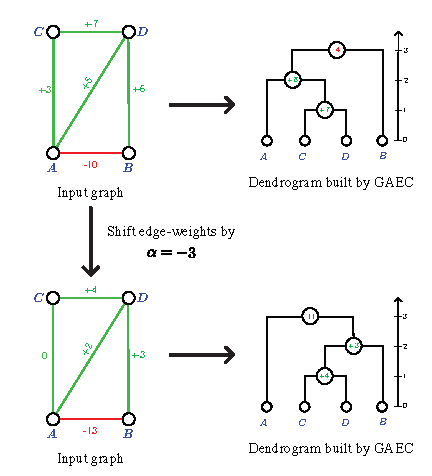
\includegraphics[width=0.48\textwidth,trim=0in 0in 0in 0in,clip]{./figs/counter-examples/counter-example-GAEC.pdf}
% \caption{Original graph and dendrogram}
% \end{subfigure}

% \vspace{2em}
% \begin{subfigure}[t]{0.48\textwidth}
% \centering
% \includegraphics[width=\textwidth,trim=0in 0in 0in 0in,clip]{./figs/counter-examples/counter-example-GAEC-shifted.pdf}
% \caption{Graph with shifted edge-weights ($\alpha=-3$) and GAEC dendrogram}
% \end{subfigure}
        \caption{ Counter-example showing that GAEC is not weight-shift invariant.
        } \label{fig:counter_examples_shift_inv_GAEC}
\end{figure}
\begin{figure}[t!]
% \begin{subfigure}[t]{0.48\textwidth}
\centering
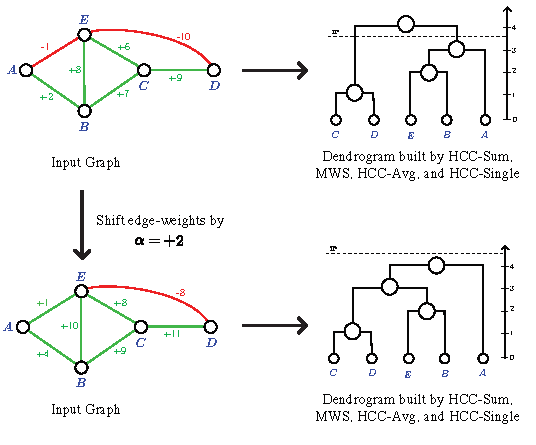
\includegraphics[width=0.48\textwidth,trim=0in 0in 0in 0in,clip]{./figs/counter-examples/counter-example.pdf}
% \caption{Original graph and dendrogram}
% \end{subfigure}

% \vspace{2em}
% \begin{subfigure}[t]{0.48\textwidth}
% \centering
% \includegraphics[width=\textwidth,trim=0in 0in 0in 0in,clip]{./figs/counter-examples/counter-example-shifted.pdf}
% \caption{Graph with shifted edge-weights ($\alpha=+2$) and dendrogram}
% \end{subfigure}
        \caption{ Counter-example showing that HCC-Sum, MWS, HCC-Avg, and HCC-Single are not weight-shift invariant.
        } \label{fig:counter_examples_shift_inv}
\end{figure}

\invariantAlgs*
\begin{proof}
Theorem 1 in \cite{chehreghani2020hierarchical} proves that hierarchical clustering with Average (HC-Avg), Single (HC-Single), and Complete linkage (HC-Complete) are weight-shift invariant.

The same is not true for \algname{} with Sum linkage criteria (GAEC and HCC-Sum), because by adding a constant $\alpha$ to all edge weights $w_e$, the interaction between two clusters $S_i$ and $S_j$ is increased by a factor $\alpha |E_{ij}|$, which depends on the number of edges  $|E_{ij}|$ connecting the two clusters. Thus, when all edge weighs of the graph are shifted, the agglomeration order may change. For a simple example of this, it is enough to consider the toy graph in Fig.~\ref{fig:intro_figure}a and shift the weights of the graph by $\alpha=-3$ (see Fig.~\ref{fig:counter_examples_shift_inv_GAEC}).


The constrained versions of \algname{} (HCC-Avg and HCC-Single) are also not weight-shift invariant: here, the algorithm merges or constrains clusters in a given order, depending on the absolute interactions $|\interact{}(S_i \cup  S_j)|$ between clusters; so, when edge weights are shifted by a constant $\alpha$, the sorting by absolute value can change arbitrarily together with the agglomeration order, as we show in the counter-example of Fig.~\ref{fig:counter_examples_shift_inv}.
Similarly, the Mutex Watershed algorithm is not weight-shift invariant because it uses a linkage criterion that compares weights by their absolute values (see again counter-example in Fig.~\ref{fig:counter_examples_shift_inv}.
\end{proof}

% \subsubsection{Ultrametrics defined by \algname{}} 



\begin{restatable}{prop}{firstUltraMetricProperty}
\label{prop:ultraMetric1}
Consider a graph $\mathcal{G}(V,E,w_e)$, a linkage criterion $\interact{}$, and an agglomerative algorithm returning a binary rooted tree $T$ with height $h_T$. Then, $(V, d_{T})$ defined in Eq.~\ref{eq:UM_def} is an ultrametric if and only if the following is true:
 % iff the interaction $\interact{}_{T}(u, v)$ associated to the least common ancestor ${(u\vee v)\in T}$ is both lower than the interaction of any other $(u\vee v)$-descendant node and higher than the interaction of any other $(u\vee v)$-ancestor node in the tree $T$. In formulae, this is equivalent to saying that, $\forall u,v,t \in V$:
\begin{gather}
\forall u,v,t \in V \nonumber \\
 h_T(u, v) < h_T(u, t) \Rightarrow \interact{}_{T}(u,v) \geq \interact{}_{T}(u,t) \label{eq:UM_assumption}
 % h_T(u, v) < h_T(u, t) \Leftrightarrow \interact{}_{T}(u,v) > \interact{}_{T}(u,t). 
\end{gather}
In words, condition \ref{eq:UM_assumption} means: if the algorithm merges nodes $u,v$ before to merge nodes $u,t$, then the signed interaction $\interact{}_{T}(u,v)$ between $u$ and $v$ has to be higher or equal than $\interact{}_{T}(u,t)$.
% In words, $(V, d_{T})$ is an ultrametric iff the interaction $\interact{}_{T}(u, v)$ associated to the least common ancestor ${(u\vee v)\in T}$ is both lower than any other $(u\vee v)$-descendant node and higher than any other $(u\vee v)$-ancestor node in the tree $T$.
\end{restatable}
\begin{proof}
% Let us first analyze assumption \ref{eq:UM_assumption}. From $(\Rightarrow)$, we have that:
% \begin{equation}\label{eq:assumption_side_1}
% h_T(u \vee v) < h_T(u \vee t) \Rightarrow \interact{}_{T}(u,v) > \interact{}_{T}(u,t). 
% \end{equation}
% In words, if the algorithm first merges node $v$ together with node $u$ and later on merges node $t$ with node $u$, then the signed interaction $\interact{}_{T}(u,v)$ between $u$ and $v$ has to be stronger than $\interact{}_{T}(u,t)$. On the other hand, the $(\Leftarrow)$ side of Eq.~\ref{eq:UM_assumption} can be rewritten as:
% \begin{equation}\label{eq:assumption_side_2}
% h_T(u \vee v) \geq h_T(u \vee t) \Rightarrow \interact{}_{T}(u,v) \leq \interact{}_{T}(u,t).
% \end{equation}
% % which in words means: if node $t$ was merged with $u$ at the same or at an earlier iteration  together with node $u$ and later on merges node $t$ with node $u$, then the interaction $\interact{}_{T}(u,v)$

From the definition of $d_{T}$, it follows that:
\begin{align}
d_{T}(u,u) &= 0 \qquad &\forall u\in V \label{eq:dist_1} \\ 
d_{T}(u,v) &\geq 0 \qquad &\forall u,v \in V \label{eq:dist_2}\\
d_{T}(u,v)& =d_{T}(v,u) \qquad &\forall u,v \in V. \label{eq:dist_3}
\end{align}
 % $d_{T}(u,v)=d_{T}(v,u)$, $d_{T}(u,u)= 0$, and $d_{T}(u,v)\geq 0$ for each $u,v \in V$.
In order to show that $(V, d_{T})$ is an ultrametric, we only need to prove the ultrametric property:
\begin{equation}\label{eq:UM_property_original}
d_T(u,v) \leq \max \{d_T(u,t), d_T(v,t)\} \quad \forall u,v,t \in V.
\end{equation}
When at least two of the three nodes $u,v,t \in V$ are the same, this property follows from Eq.~\ref{eq:dist_1} and Eq.~\ref{eq:dist_2}. When nodes $u,v,t\in V$ are distinct, from the definition of $d_{T}$ it follows that Eq.~\ref{eq:UM_property_original} is equivalent to:
\begin{equation}\label{eq:UM_property}
\interact{}_{T}(u,v) \geq \min \{\interact{}_{T}(u,t), \interact{}_{T}(v,t)\}.
\end{equation}
In the following, we prove both sides of the \emph{if and only if} statement in the proposition. First, we prove the $(\Leftarrow)$ side, i.e. that if assumption \ref{eq:UM_assumption} holds, then $(V, d_{T})$ is an ultrametric and \ref{eq:UM_property} holds. 

Case 1: in Eq.~\ref{eq:UM_property}, $t\in V$ is part of the sub-tree ${T[u \vee v]}$. In other words, the algorithm first merges node $t$ with either node $u$ or $v$, and then $u$ and $v$ are merged together. Let us assume that $t$ is first merged with $u$ (the following proof also holds for the opposite case in which $t$ is first merged with $v$):
\begin{equation}\label{eq:case_1}
h_T(u, t) < h_T(u, v) = h_T(v, t).
\end{equation}
Thus, by combining the last equation with assumption (\ref{eq:UM_assumption}), it follows that
\begin{equation}
\interact{}_{T}(u, t) \geq \interact{}_{T}(v, t) \quad  \text{and} \quad \interact{}_{T}(u, v) = \interact{}_{T}(v, t)
\end{equation}
and Eq.~\ref{eq:UM_property} follows (becoming an equality in this case).

Case 2: in Eq.~\ref{eq:UM_property}, $t\in V$ is \emph{not} part of the sub-tree ${T[u \vee v]}$. Thus, the algorithm first merges nodes $u$ and $v$, and then it merges node $t$ together with the cluster containing $u$ and $v$:
\begin{equation}
h_T(u, v) < h_T(u, t) = h_T(v, t).
\end{equation}
Thus, from assumption \ref{eq:UM_assumption} we have that
\begin{equation}
\interact{}_{T}(u, v) \geq \interact{}_{T}(u, t) \quad  \text{and} \quad \interact{}_{T}(u, v) \geq \interact{}_{T}(v, t),
\end{equation}
so also in this case Eq.~\ref{eq:UM_property} follows.
% for every distinct $u,v,t\in V$. In other words, given two leaves nodes $u,v\in V$, the depth $\interact{}_{T}(u,v)$ associated to their least common ancestor $i\in T$ should be both lower than the depth of any $i$-descendant node in $T$ and higher than any $i$-ancestor node in $T$:
%  % that have the most positive interaction   two clusters merged by the algorithm will always have an interaction that is more negative as compared to all clusters already merged and more positive than all clusters that will be merged at later iterations of the algorithm.
% \begin{equation}
% \interact{}_{T}(u,v) \geq \interact{}_{T}(u,t) \Leftrightarrow T[u \vee t] \subseteq T[u \vee v] 
% \end{equation}
%  This happens only if, at every iteration, Algorithm \ref{main_alg} merges pairs of clusters with lower and lower interactions, which is true for only certain choices of linkage criteria. %In the next section \ref{sec:alg_update_rules}, we will show that this happens only for certain linkages and only when constraints are not enforced

Next, we are left to prove the $(\Rightarrow)$ side of the \emph{if and only if} statement: if $(V, d_{T})$ is an ultrametric, then assumption \ref{eq:UM_assumption} holds.
To prove this statement, we first rephrase it in the following equivalent form: if assumption \ref{eq:UM_assumption} does not hold, then $(V, d_{T})$ is not an ultrametric and \ref{eq:UM_property} does not hold. If we negate assumption \ref{eq:UM_assumption}, there must be at least three $u,v,t \in V$ such that: 
\begin{equation}
h_T(u, v) < h_T(u, t) \quad \text{and} \quad  \interact{}_{T}(u,v) < \interact{}_{T}(u,t).
\end{equation}
The first condition, in words, is again assuming that the algorithm first merges nodes $u$ and $v$, and later it also merges node $t$ with the cluster containing $u$ and $v$. Thus, we can rephrase this assumption as:
\begin{equation}
\interact{}_{T}(u, v) < \interact{}_{T}(u, t) = \interact{}_{T}(v, t).
\end{equation}
From this, it follows that
\begin{equation}
\interact{}_{T}(u, v) < \min \{\interact{}_{T}(u, t), \interact{}_{T}(v, t)\},
\end{equation}
which is exactly the negation of the ultrametric property \ref{eq:UM_property}.
\end{proof}

\secondUltraMetricProperty*
\begin{proof}
Thanks to Prop.~\ref{prop:ultraMetric1}, we know that $(V, d_{T^*})$ is an ultrametric if and only if assumption \ref{eq:UM_assumption} holds. Thus, in the following, we will prove which variations of the \algname{} Algorithm \ref{main_alg} satisfy assumption \ref{eq:UM_assumption}. 
In other words, we need to prove in which cases \algname{} merges clusters according to a monotonously decreasing order of signed interactions $\interact{}$.

\algname{} puts clusters in a priority queue (Algorithm \ref{main_alg}, lines 5 and 15) and merges them starting from those with the highest interaction (lines 9, 19, and 26). However, the priority queue is updated each time two clusters are merged (lines 10, 20, and 27). Thus, to ensure a monotonously decreasing merging order, updated interactions involving a merged cluster should always be lower or equal than previously existing interactions (\textbf{condition 1}):
\begin{align}\label{eq:condition1}
& \forall S_i \in \Pi \setminus \{S_1, S_2\}, \nonumber \\
\interact{}(S_1 \cup S_2 \cup  S_i) &\leq \max \{ \interact{}(S_1  \cup  S_i), \interact{}(S_2  \cup  S_i)\} 
\end{align}
where $\Pi$ is a clustering, $\interact{}$ is a linkage criteria, and $S_1,S_2\in \Pi$ are two clusters merged by the algorithm at a given iteration. If this condition is true then, in the following iterations, \algname{} can only merge clusters with lower (or equal) interaction values. 

We also note that, in phase 1, the algorithm skips interactions that are both positive and constraint (condition at line 8 in Algorithm \ref{main_alg}) and merges them only later in phase 2 (line 19), when constraints are removed.
Clearly, whenever this happens, a decreasing merging order is no longer ensured. 
Thus, on top of condition 1, we also have that no merging decisions should be ``delayed'' from phase 1 to phase 2 (\textbf{condition 2}). 

Condition 1 always holds for Average, Single, Complete, and AbsMax linkage criteria, but not for a Sum linkage criteria, because the sum of two positive numbers $a,b$ is always higher than $\max\{a,b\}$. This is also demonstrated in the toy example of Fig.~\hyperref[fig:intro_figure]{\ref*{fig:intro_figure}a}, proving that, in general, Sum-linkage algorithms like GAEC or HCC-Sum do not define an ultrametric on the graph.

Thanks to Lemma \ref{lemma:absMax_and_complete_property}, we have that condition 2 always holds for algorithms based on AbsMax and Complete linkage, proving that the Mutex Watershed and HC-Complete algorithms define an ultra-metric (whether or not cannot-link-constraints are enforced). On the other hand, condition 2 does not hold for other variations of \algname{} involving cannot-link-constraints (HCC-Sum, HCC-Avg, and HCC-Single), which do not then define an ultrametric. 

Finally, the remaining not constrained versions of \algname{} (HC-Avg, HC-Single, and HC-Complete) satisfy both conditions, so they define an ultrametric, confirming the well-known results of related work in hierarchical clustering on unsigned graphs \cite{johnson1967hierarchical,milligan1979ultrametric}.

% In formulae, this can be formulated as following. Assume that at iteration $i$ \algname{} merges clusters $S_i\in \Pi$ and $S_j\Pi$ resulting in a new clustering $\Pi'=\Pi \cup \{S_i\cup S_j\} \setminus \{S_i, S_j\}$ 


% Initially, all the interactions between clusters are inserted into a priority queue (PQ) and the algorithm starts merging clusters with the highest interaction first. However, in the following iterations, 

% Since all three phases of \algname{}, the algorithm insert interactions into a priority queue and, at every iteration, picks
% - GASP merges clusters starting from those with the highest positive interaction W.
% However, assumption 5 holds only if both of the following conditions are true

% Condition 1: interaction between two merged clusters is never higher than before
% Condition 2: Positive and constrained interactions are not merged in phase 1 and "delayed" to phase 2 of the algorithm

% \emph{Average, Single, and Complete Linkage} -- 

% Given a signed graph, we can shift all edge weights by a constant $\alpha$ until they all become positive and, thanks to Prop.~\ref{prop:weight_shift_invariant}, we know that if we run hierarchical clustering (HC) with Avg, Single, or Complete linkage then the structure of the dendrogram (and the agglomeration order) will be the same for both the original signed graph and the weight-shifted positive graph. On positive weighted graphs, hierarchical clustering with any of these three linkage criteria is well known to define an ultrametric \cite{johnson1967hierarchical,milligan1979ultrametric}. Thus, if assumption \ref{eq:UM_assumption} holds for the weight-shifted positive graph $\mathcal{G}_{\alpha}$, it also has to hold for the original signed graph $\mathcal{G}$, because all interactions between clusters are simply shifted by a constant:
\end{proof}

% \subsection{Predicting signed edge weights with a CNN}
% Our CNN model outputs affinities in the form of pseudo-probabilities $p:E \rightarrow [0,1]$, where $p=0$ represents a boundary evidence. In order to use them as input of the algorithms in our framework, we mapped them to positive and negative values\footnote{Note that in general attractive and repulsive interactions $w^+$ and $w^-$ can be independently estimated with different classifiers.}. The most common approaches use \emph{additive} \cite{ailon2008aggregating} or \emph{logarithmic} \cite{finkel2008enforcing,andres2012globally} mappings:
% \begin{align} 
% \cost_{e,\mathrm{Add}} =&\,\, p_e - \beta, \\
% \cost_{e,\mathrm{Log}} =&\,\, \log \left( \frac{p_e}{1-p_e} \right) - \log \left( \frac{\beta}{1-\beta} \right), \label{eq:mappings}
% \end{align}
% where $\beta \in [0,1]$ is a \emph{bias} parameter that allow a tuning between over- and under-segmentation. We evaluated both of them empirically with each of the tested linkage and found that the additive mapping is the best option in all cases apart from the \emph{Sum} linkage. Note that varying the parameter $\beta$ does not usually define a hierarchy of nested clusterings, thus it is not equivalent to varying a threshold parameter in HAC. This hierarchical property is only valid for \algname{} without constraints and with \emph{Average}, \emph{Max} or \emph{Min} linkage.








\subsection{Mutex Watershed on SSBM graphs}
\begin{prop} \label{prop:MWS_on_SSBM}
Consider a graph generated by an Erd\H os-R\'enyi signed stochastic block model (SSBM) as described in Section \ref{sec:clustering_problems}, with $N$ nodes, edges added with probability $p$, sign-flip probability $\eta<0.5$, $k$ ground-truth clusters, and edge weights Gaussian-distributed with standard deviation $\sigma$. Then, at every iteration, \algname{} with Absolute Maximum linkage (or, in other words, the Mutex Watershed algorithm) always makes a mistake with at least probability $\eta$. 
\end{prop}
\begin{proof}
Thanks to Lemma \ref{lemma:absMax_and_complete_property} we know that \algname{} with Absolute Maximum linkage returns the same clustering whether or not cannot-link-constraints are used. Thus, in the following, we prove the proposition considering the version enforcing constraints.
Let us consider a generic iteration of the algorithm, where two clusters $S_\alpha$ and $S_\beta$ have the highest priority and are popped from priority queue. Then, the MWS algorithm will either merge or constrain them depending on the fact that their interaction $\interact_{\mathrm{AbsMax}}(S_\alpha  \cup S_\beta)$ is  positive or negative (note that, with AbsMax linkage, an interaction can never be positive and constrained, as shown in Lemma \ref{lemma:absMax_and_complete_property}).
By construction of the SSBM, every edge $e\in E$ in the graph has a absolute weight distributed as $|w_e|\sim \mathcal{N}(1,\sigma^2)$. Thus, every edge $e'\in(S_{\alpha} \times S_{\beta})\cap E$ connecting the two clusters has the same probability to have the highest absolute weight, and the sign of the interaction $\interact_{\mathrm{AbsMax}}(S_\alpha  \cup  S_\beta)$ will only depend on the sign of this highest edge. Therefore, the probability that the MWS merges two clusters is simply given by the fraction of positive weighted edges connecting them.

Let $\tilde{\Pi}=\{\tilde{S}_1,\ldots,\tilde{S}_k\}$ denote the ground truth clustering, and $\tilde{S}_{\alpha i}=S_\alpha\cap \tilde{S}_i$ denote the intersection between cluster $S_{\alpha}$ and a ground-truth cluster $\tilde{S}_i$.
If the generated graph is dense, i.e. $p=1$, then the total number of edges connecting clusters $S_{\alpha}$ and $S_{\beta}$ that have a true attractive or repulsive weight is (according to the ground truth labels)
\begin{equation}
\NBE^+=\sum_{i=1}^k |\tilde{S}_{\alpha i}||\tilde{S}_{\beta i}|, \quad \NBE^-=\sum_{i=1}^k \sum_{j=1,j\neq i}^k |\tilde{S}_{\alpha i}||\tilde{S}_{\beta j}|.
\end{equation}
When the edges in the graph are randomly added with a probability $p$, then the actual number of true attractive and repulsive interactions connecting the two clusters is (according to the ground truth labels):
\begin{equation}
\nBE^+ \sim \mathcal{B}(\NBE^+,p), \qquad \nBE^- \sim \mathcal{B}(\NBE^-,p), 
\end{equation}
where $\mathcal{B}(\NBE,p)$ is the binomial distribution:
\begin{equation}
\mathcal{B}(\nBE;\NBE,p) = \frac{\NBE !}{\nBE! (\NBE-\nBE)!} p^\nBE (1-p)^{\NBE-\nBE}.
\end{equation}
Here, we only assume that $\nBE^+ + \nBE^- >0$, i.e. there is at least one edge connecting the two clusters (otherwise their interaction would be zero and the MWS would not have popped them from priority queue). 

So far we have been talking about attractive and repulsive connections according to the ground truth labels. In our SSBM however every edge has a uniform probability $\eta$ to have its sign flip, so  the actual number of attractive interactions connecting the two clusters will be instead given by the sum of the true attractive interactions $\nBE^+_{\mathrm{nf}}\sim \mathcal{B}(\nBE^+,1-\eta)$ that have not been flipped, plus the true negative interactions $\nBE^-_{\mathrm{f}}\sim \mathcal{B}(\nBE^-,\eta)$ that have been flipped.
Putting everything together, given two clusters with $\nBE^+$ true attractive interactions and $\nBE^-$ true negative ones, the highest-absolute-weight edge connecting them has the following probability to be positive:
\begin{align}\label{eq:mws_prob}
 \mathbb{P}[\interact_{\mathrm{AbsMax}}&(S_\alpha  \cup  S_\beta)>0;\nBE^+,\nBE^-] = \nonumber \\
=&\sum_{\nBE^+_{\mathrm{nf}}=0}^{\nBE^+}\sum_{\nBE^-_{\mathrm{f}}=0}^{\nBE^-} 
\mathcal{B}(\nBE^-_{\mathrm{f}};\nBE^-,\eta) \mathcal{B}(\nBE^+_{\mathrm{nf}};\nBE^+,1-\eta)\cdot  \nonumber\\
& \qquad \qquad  \cdot \left(\frac{\nBE^+_{\mathrm{nf}}+\nBE^-_{\mathrm{f}}}{\nBE^+ + \nBE^-} \right) \nonumber\\
\stackrel{(*)}{=}&\frac{\nBE^+(1-\eta)+\nBE^-\eta}{\nBE^+ + \nBE^-}
\end{align}  
where in $(*)$ we used the fact that the expected value of a binomial distribution $\mathcal{B}(\nBE,\eta)$ is $\nBE \eta$.

%Now we note that this probability is always bounded in the interval $[\eta, 1-\eta]$ (or $[1-\eta, \eta]$, if $\eta>0.5$). Remarkably, these lower and upper bounds do not depend on the number of edges connecting the two clusters, i.e. $\nBE^+ + \nBE^-$ (and, thus, on the sizes of the two clusters). 
Now we note that this probability is bounded in the interval $[\eta, 1-\eta]$. So, regardless of whether the two clusters $S_\alpha$ and $S_\beta$ should be merged or constraint according to ground truth labels, the probability not to make the correct decision is always at least $\eta$.
% So weather we consider a merge or a split of the two clusters as the correct decision, in both cases the expected probability to not make that decision is at least $\eta$. Notably while the exact probabilities depend on the cluster sizes, the lower bound does not. This confirms the intuition that the MWS, unlike Sum or Avg linkage methods, cannot properly correct for sign flip noise by agglomerating larger boundaries and profiting from the law of large numbers. 
Remarkably, while the exact probability in Eq.~\ref{eq:mws_prob} depends on the number of edges connecting the two clusters $\nBE^++\nBE^-$ and thus on the cluster sizes, the bounds do not. Thus, this result shows that, unlike Sum or Avg linkage methods, the MWS algorithm is unable to reliably correct for the sign flip noise even for big clusters linked by many edges.
\end{proof}

% \subsection{Mutex Watershed on SSBM graphs}
% \textbf{Proposition} \\
% Consider a graph generated by an Erd\H os-R\'enyi signed stochastic block model as described in section 4 and let $S, S'$ be two clusters occurring during the agglomeration of this graph using the MWS algorithm. The expected probability that the MWS assigns a positive interaction to the boundary between those clusters is bounded by $\eta \leq P\big(\interact(S,S')>0\big) \leq 1-\eta$ where $\eta$ is the sign flip probability of the SSBM.


% \textbf{Proof} \\
% Let us write the two clusters as $S=(s_1, ..., s_k)$ and $S'=(s'_1, ..., s'_k)$ where $s_i$ indicates the number of nodes in cluster S belonging to GT-colour i. In the MWS algorithm the interaction $\interact(S,S')$ between the two clusters is determined only by the one edge with the highest absolute weight. By construction of the SSBM, every single edge in the boundary has the identical probability of having the highest absolute weight. The probability that the MWS assigns a positive interaction to the boundary between those cluster is therefore simply the fraction of positive weighted edges in the boundary. 
% The expected total number of edges in the boundary is $E_{SS'}=p|S||S'|=p\sum_{i=1}^{k}s_i \sum_{i=1}^{k}s'_i$ where p is the probability for each individual edge to be present in the graph. An edge in this boundary is positive if it either connects two nodes of the same GT-colour and did not have its sign flipped or if it connects two nodes of different GT-colors and did have its sign flipped. We can write the expected number of positive edges as $P_{SS'}=p\big(\sum_{i=1}^{k}s_is'_i\big)(1-\eta)+p\big(\sum_{i=1}^{k}s_i \sum_{i=1}^{k}s'_i - \sum_{i=1}^{k}s_is'_i\big)\eta$. The expected probability can then be written as 
% \begin{equation}
%     P\big(\interact(S,S')>0\big)=\eta +  \frac{\big(\sum_{i=1}^{k}s_is'_i\big)(1-2\eta)}{\sum_{i=1}^{k}s_i \sum_{i=1}^{k}s'_i}
% \end{equation}
% For $\eta <0.5$ this probability is bounded by $\eta \leq P\big(\interact(S,S')>0\big) \leq 1-\eta$. \\
% So weather we consider a merge or a split of the two clusters as the correct decision, in both cases we do not make that decision with a probability of at least $\eta$. Notably while the exact probabilities depend on the cluster sizes, the lower and upper bound do not. This confirms the intuition that the MWS, unlike Sum or Avg linkage methods, cannot properly correct for sign flip noise by agglomerating larger boundaries and profiting from the law of large numbers. 

% \textbf{Proof} \\
% At any given iteration, the MWS considers the boundary between two clusters $S$ and $S'$ and either merges or splits these clusters, based on the sign of the interaction $\interact(S,S')$. The algorithm employs an absolute maximum linkage criterion, the interaction $\interact(S,S')$ between the two clusters is determined only by the one edge with the highest absolute weight. By construction of the SSBM, every single edge in the boundary has the identical probability of having the highest absolute weight. The probability that the MWS assigns a positive interaction to the boundary between those cluster is therefore simply the fraction of positive weighted edges in the boundary. \\
% Let us write the two clusters as $S=(s_1, ..., s_k)$ and $S'=(s'_1, ..., s'_k)$ where $s_i$ indicates the number of nodes in cluster S belonging to GT-colour i. The expected total number of edges in the boundary is $E_{SS'}=p|S||S'|=p\sum_{i=1}^{k}s_i \sum_{i=1}^{k}s'_i$ where p is the probability for each individual edge to be present in the graph. An edge in this boundary is positive if it either connects two nodes of the same GT-colour and did not have its sign flipped or if it connects two nodes of different GT-colors and did have its sign flipped. We can write the expected number of positive edges as $P_{SS'}=p\big(\sum_{i=1}^{k}s_is'_i\big)(1-\eta)+p\big(\sum_{i=1}^{k}s_i \sum_{i=1}^{k}s'_i - \sum_{i=1}^{k}s_is'_i\big)\eta$. The expected probability can then be written as 
% \begin{equation}
%     P\big(\interact(S,S')>0\big)=\eta +  \frac{\big(\sum_{i=1}^{k}s_is'_i\big)(1-2\eta)}{\sum_{i=1}^{k}s_i \sum_{i=1}^{k}s'_i}
% \end{equation}
% For $\eta <0.5$ this probability is bounded by $\eta \leq P\big(\interact(S,S')>0\big) \leq 1-\eta$. \\
% So weather we consider a merge or a split of the two clusters as the correct decision, in both cases the expected probability to not make that decision is at least $\eta$. Notably while the exact probabilities depend on the cluster sizes, the lower bound does not. This confirms the intuition that the MWS, unlike Sum or Avg linkage methods, cannot properly correct for sign flip noise by agglomerating larger boundaries and profiting from the law of large numbers. 

% \begin{prop}\label{prop:MWS_SSBM_1}
% Consider a graph $\mathcal{G}(V,E)$ generated with a SSBM with parameters $N,p,k,\sigma$ and an associated ground truth (GT) clustering $\hat{\Pi}=\{\hat{S}_1, \ldots, \hat{S}_k\}$. Then, assume that after some merging-iterations of the MWS algorithm the clustering $\Pi$ is found. Then, any two clusters $S_i,S_j\in \Pi$ have probability $|E_{ij}| / |E_{\Pi}^1|$ to be selected in the next iteration of the algorithm, where $E_{\Pi}^1$ is the multicut associated to $\Pi$ and $E_{ij}\equiv(S_i\times S_j)\cap E$ is the set of edges connecting the two clusters. 
% \end{prop}

% \begin{prop}\label{prop:MWS_SSBM_2}
% Given the assumptions of Prop.~\ref{prop:MWS_SSBM_1}, let $E_{ij}^+=\{(u,v) \in E_{ij} | \exists \hat{S}\in \hat{\Pi} \, \mathrm{s.t.} \, u\in \hat{S} \wedge v\in \hat{S} \}$ denote the set of true attractive GT edges connecting two clusters $S_i,S_j$
% \begin{equation}
% \sum_{ij} \frac{|E_ij^+|}{||}
% \end{equation}
% \end{prop}

% Then, the MWS algorithm will assign highest priority to 
% Among these edges, we define the set of true attractive GT edges as . Finally, let $f^+=|E_{ij}^+| / |E_{ij}|$ denote the fraction of true attractive edges. Then, the Mutex Watershed algorithm 


% \begin{itemize}
% \item each pair of clusters $S_i,S_j$ has probability $|E_{ij}| / |E_{\Pi}^1|$ to have the interaction with highest priority 
% \item if the pair of clusters $S_i,S_j$ is given the highest priority by the MWS Algorithm, then they have has a probability $p^+=f^+(1-\eta) + f^+ \eta$ to be merged and $p^-=1-p^+$ to be constrained.
% \end{itemize}
% will assign a positive interaction to clusters $S_i,S_j$ with probability $f^+(1-\eta) + f^+ \eta$. 
% Remarks: this quantity does not depend on the size of $|E_{ij}|$ (so it won't change when clusters grow in size); if $f^+=1$ (i.e. $S_i,S_j$ are subclusters of the same GT cluster), then MWS will merge them with probability $1-\eta$; if $f^+=0$ (i.e. $S_i,S_j$ are subclusters of two different GT clusters), then MWS will merge them with probability $\eta$.
% \TODO{Assumption about $\sigma$?}


\subsection{Application to neuron segmentation}\label{sec:cremi_details}
\paragraph{Training and data augmentation} The data from the CREMI challenge is highly anisotropic and contains artifacts like missing sections, staining precipitations and support film folds. 
To alleviate difficulties stemming from misalignment, we use a version of the data that was elastically realigned by the challenge organizers with the method of \cite{saalfeld2012elastic}.
% We train a 3D U-Net \cite{ronneberger2015u,cciccek20163d} using the same architecture as \cite{funke2018large} and predict the same set of long-and-short range affinities described in \cite{lee2017superhuman}. 
In addition to the standard data augmentation techniques of random rotations, random flips and  elastic deformations, we simulate data artifacts.
We randomly zero-out slices, decrease the contrast of slices, simulate tears, introduce alignment jitter and paste artifacts extracted from the training data. Both \cite{funke2018large} and \cite{lee2017superhuman} have shown
that these kinds of augmentations can help to alleviate issues caused by EM-imaging artifacts.
We use L2 loss and Adam optimizer to train the network. The model was trained on all three samples with available ground truth labels.  

\paragraph{CREMI-gridRag instances} 
Our 3D UNet model predicts the same set of 12 long-and-short range affinities as described in \cite{lee2017superhuman}. 
When building the pixel-grid graph, we add both direct neighbors connections and the long-range connections predicted by our model (every voxel is connected to other six voxels via direct connections and other 18 voxels via long-range edges).
Empirically, when long-range predictions of the CNN are added as long-range connections in the graph, \algname{} achieves better scores as compared to when only direct-neighbors predictions are used.
% Empirically, we found that adding only 10\% of the long-range connections to the grid-graph (by sampling them at random) gave the best results.
Our intuitive explanation of this is that, where there is a clear boundary evidence between two segments, the long-range predictions of the CNN model are more certain than the direct-neighbor ones, because it is often impossible to estimate the exact ground-truth label transition for pixels that are very close to a boundary evidence. 
However, empirically, we also find that \algname{} achieves the best scores when only 10\% of the long-range connections are randomly sampled and added to the grid-graph. When all the long-range connections predicted by the CNN are added to the graph (18 connections for every voxel), all versions of \algname{} tend to perform more over-clustering errors.
In practice, we explain this by observing that many challenging parts of the studied neuron segmentation data involve thin and elongated segments, and our model sometimes fails to connect distant pairs of pixels that, according to the ground-truth labels, should belong to the same segment (even though, in this case, the direct neighboring predictions are correct).
To sum up, the scores we report in Tables \ref{tab:scores_gridGraph} are obtained by using only 10\% of the long-range predictions, since this was the setup that performed the best.
After running \algname{}, we use a simple post-processing step to delete small segments on the boundaries, most of which are given by single-voxel clusters. On the neuron segmentation predictions, we deleted all regions with less than 200 voxels and used a seeded watershed algorithm to expand the bigger segments.



\paragraph{CREMI-3D-rag instances} 
We build these clustering problems by generating superpixels and then building a 3D region adjacency graph.
Due to the anisotropy of the data, we generate 2D superpixels by considering each 2D image in the stack singularly.
First, we generate a boundary-evidence map by taking an average over the two direct-neighbor predictions of the CNN model (one for each direction in the 2D image of the stack) and applying some additional smoothing. Then, we threshold the boundary map, compute a distance transform, and run a watershed algorithm seeded at the maxima of the distance transform (WSDT). The degree of smoothing was optimized such that each region receives as few seeds as possible, without however causing severe under-segmentation. 
The computed 2D superpixels are then used to build a 3D region-adjacency graph (3D-rag). The weights of the edges are given by averaging the CNN affinities over the boundaries of adjacent superpixels. 

% \paragraph{Lifted Multicut pipeline}
% Similarly to what explained in the previous paragraph, we compute 2D superpixels using the WSDT procedure and build a 3D region-adjacency graph. The weights of the edges connecting neighboring superpixels are computed by taking an average over both short- and long-range affinities connecting the two regions. 
% We then convert the edge probabilities to signed weights using the logarithmic mapping defined in Eq. \ref{eq:mappings} and solve the multicut problem on this graph. For our experiments, we use the approximate Kernighan-Lin solver \cite{keuper2015efficient,kernighan1970efficient} (WSDT+MC). In some cases, the long-range affinities predicted by the CNN can connect two superpixels that are not direct-neighbors. Thus, in these cases we introduce additional \emph{lifted} edges in the graph and an instance of the lifted multicut problem (WSDT+LMC). This time, similarly to the methods mentioned in \cite{beier2016efficient}, we used a combination of approximate solvers consisting of GAEC and Kernighan-Lin. 



% \subsection{\algname{} on the full CREMI dataset} \label{sec:appendix_exps_full_cremi}
 % \paragraph{Pre-merge processing} For the predictions on the full dataset from the CREMI challenge, we used  the padded volumes provided by the challenge. The crops on which we performed a prediction have a size of $1500\times1500\times127=2.86\cdot 10^8$ voxels or larger. Building a graph with $10^8$ nodes can easily incur a large use of memory, so we decided to perform a preprocessing step by initially merging some nodes together. Simply down-sampling the predictions of the CNN would have led to a loss of resolution and performances in the most difficult parts of the dataset. Thus, we decided to pre-merge the most connected components of the graph that would be anyway clustered during the first iterations of \algname{}. To do this, we used a simple approach: we generated a boundary probability map by taking for each voxel an average over affinities in all directions (both short- and long-range ones) and we run THRESH with a conservative threshold parameter to find the connected components. With this approach, pixels are pre-clustered only when they are far away (in all directions) from predicted boundaries. 
 % To make sure that in this preprocessing step different neurons are never merged together by mistake, we intersected the segments given by THRESH with the segments given by WSDT. 
 % We tested \algname{} both on the full grid-graph and on this preprocessed graph and we did not notice any major differences in the final clustering or achieved scores, although the version with a pre-processed graph was significantly faster. To reduce the runtime and memory requirements even further, we used only 10 \% of the long-range connections in the pixel-graph, since adding all of them did not improve the scores.  
 
 
 % \paragraph{Enforcing local merge} In 2D images of urban-scenes, due to partial occlusion, one object instance can be given by multiple components that are not directly connected in the image plane. This is not the case in neuron-segmentation, where each neuron should be given by a single 3D connected component in the volume. In order to enforce it, we modified the implementation of \algname{} so that two clusters are merged only when they represent two adjacent supervoxels in the 3D volume and if this condition is not satisfied, the merge is postponed until there is a direct connection. This then avoids the introduction of ``air-bridges'' between segments due to attractive long-range connections in the initial voxel grid-graph.
 % This approach achieved superior performances to the one proposed in \cite{wolf2018mutex}, where all long-range connections in the grid-graph are associated to a negative repulsive edge weight.

% \begin{table*}[t]
% \centering
%     \scriptsize
%         \begin{tabular}{l|c|c|c|c|c}
%           \algname{} linkage & \makecell{CREMI-Score\\(lower better)}  & \makecell{Rand-Score\\(higher better)} & \makecell{VI-merge\\(lower better)} & \makecell{VI-split\\(lower better)} & \makecell{Runtime\\(lower better)} \\ \midrule
% Average & \textbf{0.226} & \textbf{0.936} & 0.315 & 0.494 & 3.49 $\cdot$ 10$^4$ \\
% Sum + CLC \cite{levinkov2017comparative} & 0.282 & 0.906 & 0.358 & 0.510 & 4.64 $\cdot$ 10$^4$ \\
% Abs Max \cite{wolf2018mutex} & 0.322 & 0.897 & 0.286 & 0.735 & 1.24 $\cdot$ 10$^4$ \\
% Max + CLC & 0.324 & 0.893 & 0.292 & 0.698 & 6.31 $\cdot$ 10$^4$ \\
% Sum \cite{keuper2015efficient} & 0.334 & 0.872 & 0.461 & 0.444 & 4.74 $\cdot$ 10$^4$ \\
% Average + CLC & 0.563 & 0.772 & 0.259  & 1.142 & 2.95 $\cdot$ 10$^4$ \\
% Min & 2.522 & 0.030 & \textbf{0.197} & 6.365 & 2.97 $\cdot$ 10$^3$ \\
% Min + CLC & 2.522 & 0.030 & \textbf{0.197}  & 6.365 & 4.77 $\cdot$ 10$^3$ \\
% Max & 2.626 & 0.028 & 7.069 & \textbf{0.026} & \textbf{6.04 $\cdot$ 10$^\mathbf{2}$} \\
%         \end{tabular}
%         \vspace*{1.1em}
%     \caption{Performances achieved by different versions of \algname{} on the CREMI 2016 training set. 
%     CREMI-Score \cite{cremiChallenge}, is given by a combination of the Adapted Rand-Score (Rand-Score) and the Variation of Information Score for under-clustering (VI-merge) and over-clustering (VI-split) \cite{arganda2015crowdsourcing}.
%     CLC stands for cannot-link constraints. For all algorithms, the chosen value of bias parameter was $\beta = 0.5$. }
%     \label{tab:extended_results_cremi}
% \end{table*}

\begin{table*}[t]
    \centering
    \scriptsize
    % \tiny
    \begin{subtable}[t!]{\textwidth}
    \centering

        \begin{tabular}{l | r r r r r r r r r}
        % \toprule
         %\multicolumn{1}{c}{}
        % &\multicolumn{5}{c}{Multicut objective values associated to final clusterings (lower is better)} \\
        Clustering problem & \multicolumn{1}{r}{GAEC \cite{keuper2015efficient}} & HCC-Sum & MWS \cite{wolf2018mutex} & HC-Avg & HCC-Avg & HC-Single & HCC-Single & HC-Complete \\ \midrule
        \emph{Modularity Clustering} & 
        -0.457 & -0.453 & -0.073 & \textbf{-0.467} & \textbf{-0.467} & 0.000 & 0.000 & -0.201 \\ 
        \emph{Image Segmentation}  & 
        \textbf{-2,955} & -2,953 & -2,901 & -2,903 & -2,896 & -1,384 & -1,384 & -2,102 \\
        \emph{Knott-3D (150-300-450)}  & 
        \textbf{-36,667} & -36,652 & -35,200 & -35,957 & -35,631 & -2,522 & -2,522 & 30,629 \\
        % \emph{Knott-3D-300} & \emph{3D-rag} & 8& & & \HollowBox\\
        % \emph{Knott-3D-450}& \emph{3D-rag} & 8 & & & \HollowBox\\  
        \emph{CREMI-3D-rag}  
        & \textbf{-1,112,287} & -1,112,286& -1,109,731 & -1,112,177 & -1,112,100 & -1,038,709 & -1,038,709 & -748,734,869 \\ 
        \emph{Fruit-Fly Level 1-4}
        & \textbf{-151,022} & -151,017 & -150,879 & -150,909 & -150,876 & -71,477 & -71,997 & -128,733 \\
        \emph{CREMI-gridGraph} 
        & -73,317,601 & -73,328,867 & -73,330,568 & \textbf{-73,502,947} & -73,474,856 & -45,194,180 &-45,194,443 & 311,598,700 \\
        \emph{Fruit-Fly Level Global} 
        & \textbf{-151,688} & -151,596 & -146,315 & -150,466 & -150,171 & -4,422 & - & 6,876 \\
        % \emph{(CREMI-pixGrid-LSIMasksUNet)} & \emph{gridGraph} & 1 & & 4 & \CrossedBox\\
        % \emph{(CityScapesValidation-pixGrid)} & \emph{gridGraph} &  &  & & \CrossedBox\\
        % \emph{CREMI-test....}\\\midrule
        % \emph{Stochastic Block Model (synthetic)} & \emph{non-planar} &-&- & - & \CrossedBox \\
        % \emph{(epinions and slashdot?)} & \emph{dense?} &  & & & \HollowBox\\ 

% fruitfly-large & -151687.891 & -151596.344 & -146315.031 & -150466.000 & -150171.203 & -4422.442 & - & 6875.726 & 6879.776 \\
% modularity-clustering & -0.457 & -0.453 & -0.073 & -0.467 & -0.467 & 0.000 & 0.000 & -0.201 & -0.201 \\
% knott & -36667 & -36652 & -35200 & -35957 & -35631 & -2522 & -2522 & 30629 & 30599 \\
% fruitfly-medium & -151022 & -151017 & -150879 & -150909 & -150876 & -71477 & -71997 & -128733 & -128732 \\
% image-seg & -2955 & -2953 & -2901 & -2903 & -2896 & -1384 & -1384 & -2102 & -2102 \\

% % Superpixels:
% Mutex & -1109731264 \\
% MEANconstr & -1112099691 \\
% MEAN & -1112176981 \\
% SUMconstrNoLogs & -1112286144 \\
% SUMnoLogs & -1112286741 \\
% MAX & -1038708864 \\
% MAXconstr & -1038708864 \\
% MIN & -748734869 \\
% MINconstr & -748766347 \\

% % Pixels:
% SUM & -73317601 \\
% SUMconstr & -73328867 \\
% MutexPixGrid & -73330568 \\
% MEANconstr & -73474856 \\
% MEAN & -73502947 \\
% MAX & -45194180 \\
% MAXconstr & -45194443 \\
% MIN & 311598700 \\
% MINconstr & 311520538 \\


        \end{tabular}
    \end{subtable} 
    \caption{We compare algorithms in the \algname{} framework by evaluating which of the obtained clusterings is associated to the lowest value of the multicut objective defined in Eq.~\ref{eq:MC_objective} (lower is better). Single and complete linkage methods performed much worse than the others. Note that HCC-Single is the algorithm with the highest runtime (see Table \ref{tab:scores_gridGraph}) and it did not scale up to the very large clustering problem \emph{Fruit-Fly Level Global}.
% We used a machine with CPU Intel(R) Xeon(R) E7-4870 @ 2.40GHz for our comparison experiments.
    } 
    \label{tab:all_multicut_energies}
\end{table*}


\subsection{Adding structured noise to CNN predictions} \label{sec:appendix_noise_gen}
Additionally to the comparison on the full training dataset, we performed more experiments on a crop of the more challenging CREMI training sample B, where we perturbed the predictions of the CNN with noise and we introduced additional artifacts like missing boundary evidences.

In the field of image processing there are several ways of adding noise to an image, among which the most common are Gaussian noise or Poisson shot noise. 
In these cases, the noise of one pixel does not correlate with its neighboring noise values. On the other hand, predictions of a CNN are known to be spatially correlated. 
Thus, we used Perlin noise\footnote{In our experiments, we used an open-source implementation of simplex noise \cite{perlin2001noise}, which is an improved version of Perlin noise \cite{perlin1985image}}, one of the most common gradient noises used in procedural pattern generation. This type of noise $n(x)\in[0,1]$ generates spatial random patterns that are locally smooth but have large and diverse variations on bigger scales. We then combined it with the CNN predictions $p(x)$ in the following way:
\begin{equation}\label{eq:noise_biased_predictions}
\tilde{F}(x;\mathcal{K})=F(x)+\mathcal{K}\cdot\max\left(N(x),0\right),
\end{equation}
where  $N(x)=\mathrm{Logit}[n(x)]$; $F(x)=\mathrm{Logit}[p(x)]$ and $\mathcal{K}\in \mathbb{R}^+$ is a positive factor representing the amount of added noise. The resulting perturbed predictions $\tilde{F}(x;\mathcal{K})$ are then under-clustering biased, such that the probability for two pixels to be in the same cluster is increased only if $N(x)>0$ (see Fig.~\hyperref[fig:noisy_affs]{\ref*{fig:noisy_affs}b} and \hyperref[fig:noisy_affs]{\ref*{fig:noisy_affs}c}). 
% whereas $\tilde{F}_{-}(x;\mathcal{K})$ is a over-clustering biased prediction with decreased probabilities when $N(x)<0$ (Fig. \hyperref[fig:noisy_affs]{\ref*{fig:noisy_affs}c}).
Note that in these experiments we focused only on predictions perturbed with under-clustering biased noise (and not over-clustering biased noise). The reason is that generating realistic over-clustering biased CNN predictions is more complex and cannot be simply done by adding Perlin noise: as we show in Fig.~\hyperref[fig:noisy_affs]{\ref*{fig:noisy_affs}c}, by adding Perlin noise we can easily ``remove'' parts of a boundary evidence, but it is not possible to generate random new realistic boundary evidence.  
% In the implementation we used, the noise can be generated in an arbitrary number of dimensions and a smoothing factor can be specified for each direction independently. 

In our experiments, each pixel is represented by a node in the grid-graph and it is linked to $n_{\mathrm{nb}}$ other nodes by short- and long-range edges. Thus, the output volume of our CNN model is a four-dimensional tensor with $n_{\mathrm{nb}}$ channels: for each pixel / voxel, the model outputs $n_{\mathrm{nb}}$ values representing affinities of different edge connections. We then generated a 4-dimensional Perlin noise tensor that matches the dimension of the CNN output. The data is highly anisotropic, i.e. it has a lower resolution in one of the dimensions. Due to this fact, we chose different smoothing parameters to generate the noise in different directions. 
% \TODO{Give these smoothing parameters...}

% The experiments summarized in Fig. \ref{fig:scores_structured_noise} were performed in the following way: for each value $\mathcal{K}$, 20 random noise samples were drawn, from which median and percentiles statistics were computed for each different linkage criteria. 
% For each sample, we randomly selected some of the long-range predictions from the CNN and added them to pixel grid-graph.
\begin{figure*}[t]
\centering
        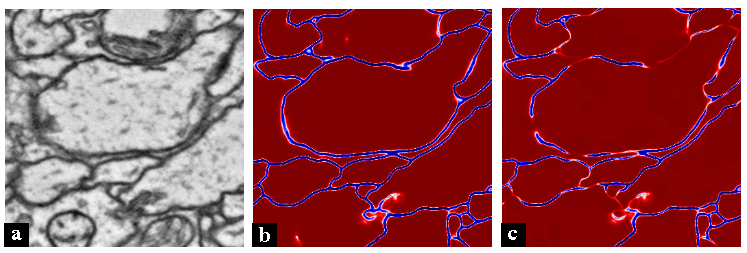
\includegraphics[width=\textwidth,trim=0.0in -0.in -0.0in -0.4in,clip]{figs/noisy_affs_comparison_v2.pdf}
    \caption{CNN predictions on a slice of the CREMI neuron segmentation challenge with and without additional spatially-correlated noise. (\textbf{a}) Raw data (\textbf{b}) Original CNN predictions $F(x)$, where blue pixels represent boundary evidence (\textbf{c}) Strongly perturbed version $\tilde{F}(x;\mathcal{K})$ of the predictions defined in Eq. \ref{eq:noise_biased_predictions} with $\mathcal{K}=8$. Long-range predictions are not shown. 
    }
    \label{fig:noisy_affs}
\end{figure*}
% \begin{table}
%     \centering
%     % \small
%     \vspace*{0.6em}
%         \begin{tabular}{l M{7em} M{7em}}
%           \algname{} linkage & AP  & Bias $\beta$ \\ \midrule
%           Average & 34.3 & 0.35 \\
%           Average + CLC & 33.9 & 0.25\\
%           Max + CLC & 32.5 & 0.50 \\
%           Abs Max & 32.1 & 0.45\\
%           Sum + CLC & 31.9 & 0.55 \\
%           Sum & 31.3 & 0.55 \\
%           Max & 24.3 & 0.85 \\
%           Min & 0.00 & 0.50 \\
%           Min + CLC & 0.00 & 0.50 \\
%         \end{tabular}
%     \vspace*{2em}
%     \caption{Average Precision (AP) scores achieved by different versions of \algname{} and chosen bias parameters $\beta$ on the cityscapes validation set. A bias value $\beta=0$ returns one single cluster. CLC stands for cannot-link constraints.}
%     \label{tab:extended_results_cityscapes_val}
% \end{table}




% \subsection{Fine-tuning the GMIS pipeline on CityScapes} \label{sec:appendix_cityscapes}
% For our experiments, we used the model from GMIS \cite{liu2018affinity} that is publicly available. 
% The model consists of two neural networks with similar structures, one predicting pixel level semantic scores and the other predicting pixel affinities between instances. We also used all the affinity post-processing methods proposed in \cite{liu2018affinity}, e.g. excluding background, resizing regions of interest or the proposed "affinity-refinement" method, which combines semantic and instance outputs. 
% The instance-branch of the model was trained with a Binary Cross-Entropy loss, but we noticed how the short-range affinities were biased towards high probabilities, so that a strong short-range boundary evidence was never predicted by the model. In \cite{liu2018affinity}, they handle this problem by proposing a modified version of HAC that is done in stages (MultiStepHAC): initially only short-range affinities are used to run HAC and a low threshold in the hierarchy is chosen to define a first clustering; then a new HAC problem including long-range affinities is  initialized with the first clustering; in the method proposed by \cite{liu2018affinity}, these steps are repeated three times. 

% Since MultiStepHAC is a rather complex post-processing method that requires to tune several hyper-parameters, we opted for a different approach to solve the problem of the unbalanced affinities. We added two 1x1 convolutional layers to the instance-branch model and trained them by using the same loss used by \cite{wolf2018mutex} and is based on the S\o resen-Dice coefficient \cite{dice1945measures,sorensen1948method}. Compared to Hamming-distance based loss like Binary Cross-Entropy or Mean Squared Error, the advantage of this loss is its being robust against prediction and / or target sparsity, that is a desirable quality in this application since boundaries between instances can be sparse. 
% During training, all the affinities involving at least one pixel belonging to the background were ignored in the loss. In this way, these last two layers specialized in improving the predictions of boundary evidence between adjacent instances (especially those belonging to the same class). We then considered an average of these new fine-tuned affinities with the ones predicted by the original model. During the fine-tuning process, only the parameters of the last two convolutional layers were updated.

% Before to apply \algname{}, we performed a parameter-search for the bias $\beta$ defined in \ref{eq:mappings}. Table \ref{tab:extended_results_cityscapes_val} lists the best-case performances for each of the methods: note that depending on the \algname{} linkage criterion, it was necessary to bias more or less the predicted edge weights.

% The semantic categories are assigned to each instance in the same way proposed by \cite{liu2018affinity}, i.e. with a majority vote based on the semantic output of the model.





\begin{table*}[t]
\centering
% \begin{minipage}[t]{0.48\textwidth}
% \vspace{0pt}
% \centering
% \footnotesize
\begin{tabular}[t]{l c}
           Method & ARAND Error \\ \midrule
           \textbf{HC-Avg} (GASP with Avg Linkage) & \textbf{0.1034} \\
GAEC \cite{keuper2015efficient} (GASP with Sum Linkage) & 0.1035 \\
MWS \cite{wolf2018mutex} (GASP with AbsMax linkage) & 0.1068 \\
SPONGE$_{sym}$ \cite{Cucuringu2019SPONGEAG} & 0.4161\\
$L_{sym}$ \cite{kunegis2010spectral} & 0.8069 \\
SPONGE \cite{Cucuringu2019SPONGEAG} & 0.9211 \\
BNC \cite{chiang2012scalable} & 0.9926 \\
        \end{tabular}
    \caption{\algname{} compared to spectral clustering methods on a small crop of the CREMI neuron segmentation dataset. 
    Since spectral methods cannot scale to the full CREMI dataset, we evaluated them on a smaller $10\times100\times100$ sub-volume of CREMI training sample B.
    Despite the fact that the true number of ground truth clusters was given as an input to the spectral methods, GASP significantly outperformed them. 
    % SC methods seem to have more difficulties when the graph is sparse. 
    % Spectral methods did not handle well pixels on the boundaries between segments and tended to cluster them together. 
    % We also tried to vary the input number of clusters ncreasing $k$ did not improve their scores either.
% resulting in a graph with $10^5$ nodes and~$\sim10^6$ edges.
    }
    \label{tab:cremi_spectral_experiments}
% \end{minipage}
% \begin{minipage}[t]{0.38\textwidth}
% \vspace{0pt}
% \centering
%         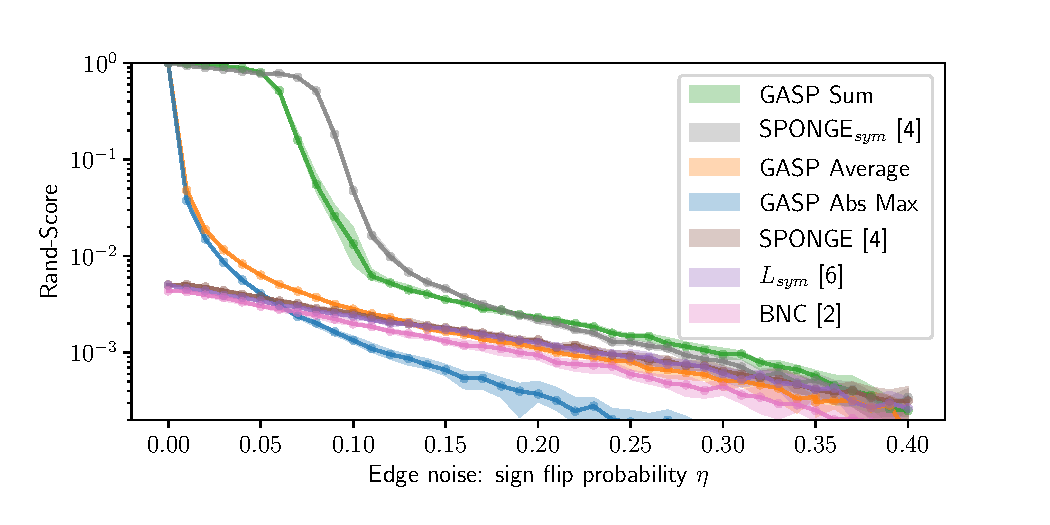
\includegraphics[width=1.\textwidth,trim=0.25in 0.25in 0.68in 0.36in,clip]{./figs/SSBM_experiments.pdf} % 0.45
%         \caption{\algname{} performances compared to spectral methods on synthetic graphs. The spectral methods were given the true number of clusters as input, in contrast to \algname{}. \TODO{Define paramters SSB; explain percentile stuff (for both noise experiments, save space!)}}
%     \label{fig:SSBM_scores}
% \end{minipage}
\end{table*}


% \subsection{Comparison with spectral clustering} \label{sec:spectral_clust}
% In this section we compare \algname{} to spectral clustering (SC) methods on signed graphs from neuron segmentation. These methods require the user to specify the number of clusters in advance, in contrast to our proposed agglomeration method that determines the cluster number based on the signed weights of the graph. In the following comparison, we make these baselines as strong as possible by specifying the true number of clusters for the spectral methods.
% % \textbf{Synthetic graphs} -- First, we compare the clustering performance on synthetic graphs generated by a signed stochastic block model (SSBM), where SC performs well. In particular, we used an Erd\H os-R\'enyi random graph model $\mathcal{G}(N,p)$ with $N=10^5$ vertices and edge probability $p=0.1$. Following the approach in \cite{Cucuringu2019SPONGEAG}, we partitioned the graph into $k=100$ equally-sized clusters, such that edges connecting vertices belonging to the same cluster (different clusters, respectively) had Gaussian distributed edge weights centered at $\mu=1$ ($\mu=-1$, respectively) and with standard deviation $0.1$. To model noise, we flipped the sign of each edge independently with probability $\eta \in [0, 0.4]$. Median scores, 25th and 75th percentiles over 30 repetitions are shown in Fig.~\ref{fig:SSBM_spectral_experiments}: GASP achieved scores comparable to SPONGE$_{sym}$ \cite{Cucuringu2019SPONGEAG}, a recently proposed SC method. The specific design choice of a \emph{sign flipping} noise used in the SSBM experiments turned out to favor GASP with \emph{Sum} linkage that, according to the experiments presented in Sec.~\ref{sec:results}, is the one with the lowest tendency to over-cluster and grows one cluster at the time.
% We extended the comparison with spectral methods to the task of neuron segmentation. Since SC cannot scale to the full CREMI dataset \TODO{}, we evaluated \algname{} and SC on a smaller $10\times100\times100$ voxels volume resulting in a graph with $10^5$ nodes and~$\sim10^6$ edges. Scores are summarized in Table \ref{tab:cremi_spectral_experiments}.
% %suggested by the reviewer that performed best in the recent comparison \cite{Cucuringu2019SPONGEAG}: one based on the Balanced Normalized Cut (BNC) \cite{chiang2012scalable}; another on the symmetrically normalized Signed Laplacian ($L_{sym}$) \cite{kunegis2010spectral}; SPONGE and SPONGE$_{sym}$ algorithms were recently proposed in \cite{Cucuringu2019SPONGEAG}.
% Despite the fact that the true number of ground truth clusters was given as an input to the SC methods, GASP significantly outperformed them on neuro-data. SC methods seem to have more difficulties when the graph is sparse. Moreover, they did not handle well pixels on the boundaries between segments and tended to cluster them together. Increasing $k$ did not improve their scores either.




